\chapter{Phase II - Design et analyse}


\section{Avant les phases II}

Avant les phases II, on a la phase I, les études PK/PD (pharmacokinetic / pharmacodynamic) et les  études précliniques.

\begin{itemize}
    \item Phase I
    \begin{itemize}
    \item MTD : Maximum Tolerated Dose : dose maximum pouvant
être administrée au patient
    \item Première idée du profil de toxicité.
\end{itemize}
\item études PK/PD (pharmacokinetic / pharmacodynamic)
\begin{itemize}
    \item Information sur l’absorption et l’élimination du traitement
     \item Permet de déterminer la dose et le schedule
d’administration pour maintenir la concentration du
traitement dans le sang, le plasma, …
\end{itemize}
\item études précliniques.
\end{itemize}



\section{Objectifs}

L'objectif de cette phase de l'essai clinique est d'évaluer l’activité thérapeutique du traitement sous une dose et un schédule déterminé et de compléter l’information disponible sur le profil de toxicité du traitement considéré. On veut savoir si l’activité du traitement est suffisant pour continuer le développement /l’investigation de ce traitement.

\section{Définition}

La définition la plus simple pour ce la phase II est 
\begin{center}
    \textbf{« It is to some extent easier to define phase II as the studies which are carried out following phase I assessment of a new agent but before large-scale assessment as part of a randomized phase III trial.}
\end{center}

Il y aussi différentes définitions/classifications ont été proposées:
\begin{itemize}
    \item Early Phase II versus Late Phase II
    \item Phase IIA versus Phase IIb
    \item Single agent Phase II versus Combined modality treatment Phase II
     \item Early Phase II versus Feasibility Phase II

\end{itemize}

\section{Analyse}

En général, on fait test d’hypothèse sur un « taux de réponse » par rapport à une norme considérée comme acceptable/inacceptable.\\
La taille d’échantillon est calculée sur base de deux taux de réponse :
\begin{itemize}
    \item P0 : le taux de succès en dessous duquel le traitement sera déclaré
inactif,
    \item P1 : le taux de succès au-dessus duquel le traitement sera déclaré
actif.
\end{itemize}

\section{Différents designs}

Il existe toute une série de designs et plusieurs améliorations/modifications ont été proposés dans la littérature.

Les plus courants sont : 
\begin{itemize}
    \item Gehan’s two stage design (1961)
    \item Fleming multiple-stage design (1982)
    \item Simon two-stage design (1989)
    \item Bryant and Day two-stage design (1995)
\end{itemize}

\subsection{Design de Gehan (1971)}
C'est un design en deux étapes et non randomisé. 

\subsubsection{étape 1}

Lors de l'étape 1, on a $n_{1}$ patients sont traités et on calcule $Y{1}$ = nombre de patients parmi les $n_{1}$ pour lesquels une activité thérapeutique du traitement a été observé (endpoint). 

On a ainsi la règle de décision :
\begin{itemize}
    \item Si Y1 = 0 on arrête l’étude et le développement clinique du traitement
    \item Si Y1 > 0 on continue l’étude
\end{itemize}
\begin{figure}[H]
    \centering
    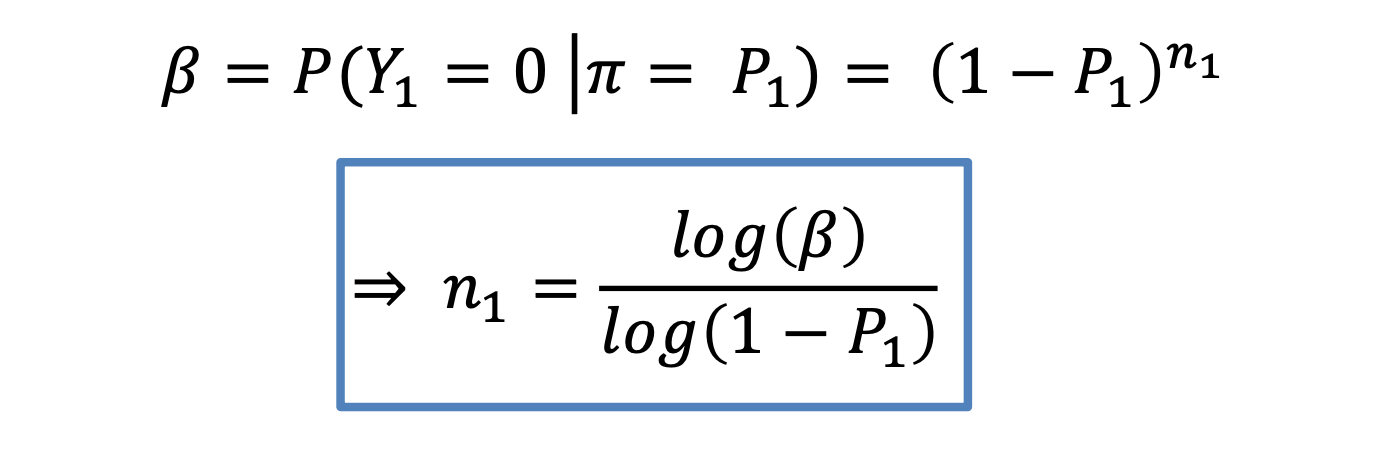
\includegraphics[scale = 0.3]{images/gehan1.png}
    \caption{Gehan: étape 1}
    \label{fig:gehan1}
\end{figure}

\subsubsection{étape 2}
n2 patients sont traités de façon à obtenir une estimation de $\pi$
avec une erreur standard maximum donnée $\sigma_{M}$ (dans
l’échantillon global : $n = n_1 + n_2$)

\begin{figure}[H]
    \centering
    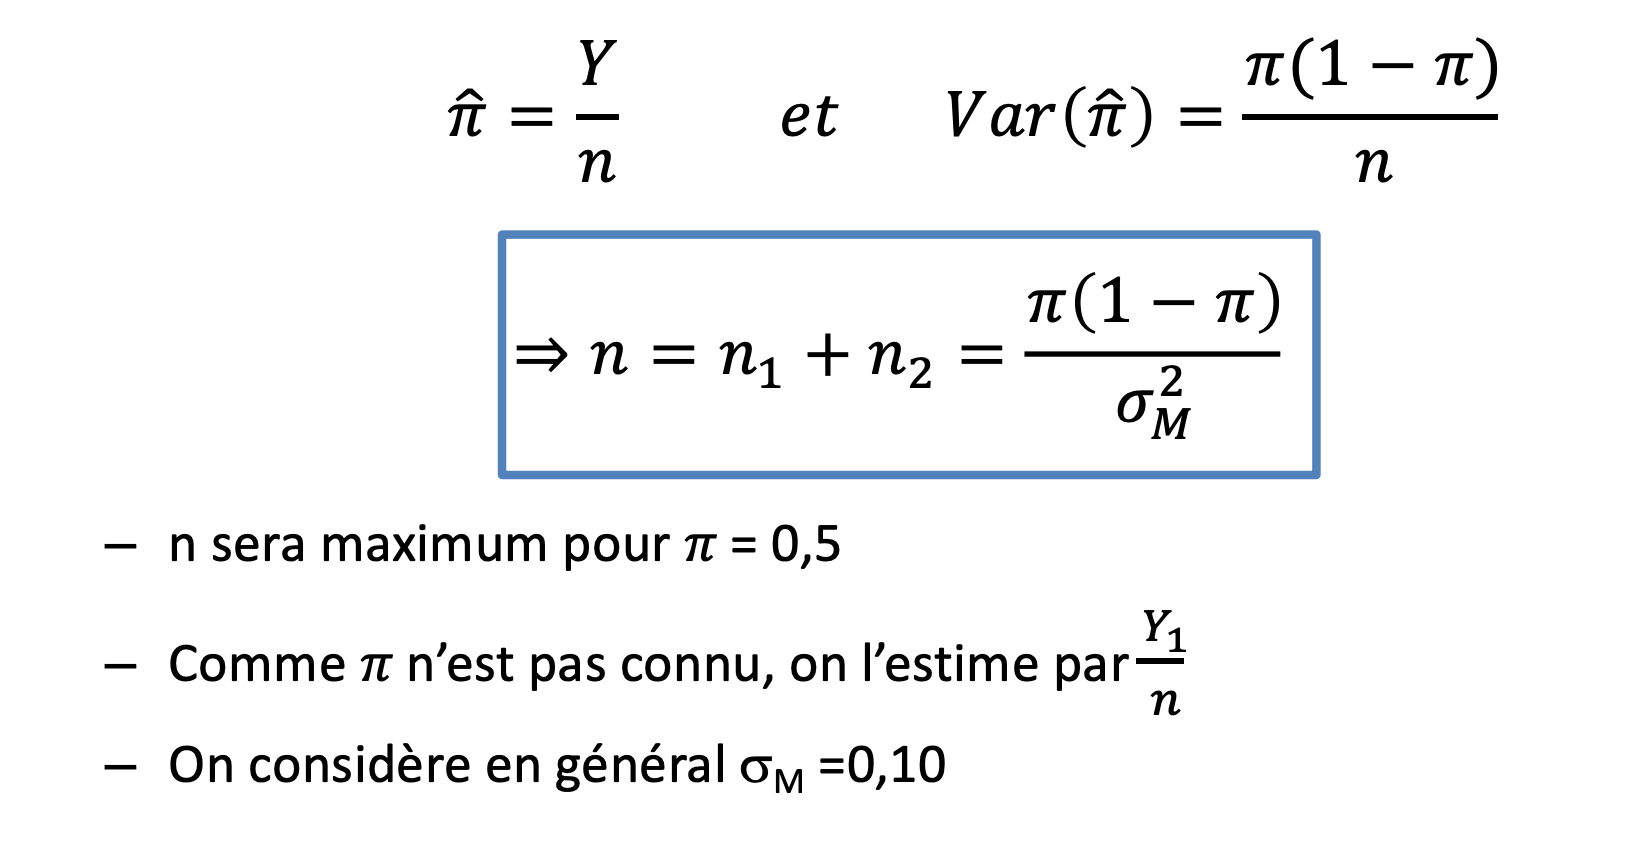
\includegraphics[scale = 0.3]{images/gehan2.png}
    \caption{Gehan: étape 2}
    \label{fig:gehan2}
\end{figure}

\subsection{Design de Fleming (1982)}
C'est une amélioration du design de Gehan. 

\subsection{Two-stage Simon design (1989)}
C'est un design en deux étapes. On considère que le traitement ne peut pas être accepté après la $1^{1}$ étape. 
\subsubsection{Étape 1}
on recrute n1 patients
\begin{itemize}
    \item Si r1 réponses ou moins : on arrête l’étude et on recommande de ne
pas poursuivre le développement
     \item Si plus de r1 réponses : on passe à l’étape 2 
\end{itemize}
\subsubsection{Étape 2}
on recrute n2 patients supplémentaires.
\begin{itemize}
    \item Si r réponses ou moins : on arrête l’étude et on recommande de ne pas
poursuivre le développement
   \item Si plus de r réponses : on arrête l’étude et on recommande de poursuivre le développement.
\end{itemize}
\subsection{Ensign design (1994)}
Le Simon design ne permet en général pas de s’arrêter tôt au cas où beaucoup d’échec sont observé en début d’étude.

\subsubsection{Idée}
\begin{itemize}
    \item Étape 1 : étape 1 d’un design de Gehan
    \item Étape 2 et 3 : Simon design 
\end{itemize}

La taille d’échantillon moyenne sera en général plus petite pour ce 3 stage design que pour le Simon two-stage.
\subsection{Bryant and Day design (1995)}
C'est un design similaire par sa structure au Simon design, mais on
évalue à la fois la réponse et la toxicité.

On peut utiliser ce type de design pour des traitements pour lesquels le profil de toxicité est peu connu. Par exemple :
\begin{itemize}
    \item Traitement pour lequel le concept de « phase I » n’a pas vraiment de
sens (par exemple radiothérapie, chirurgie, …)
\item Pas vraiment d’information « utilisable » venant des phases I (autre
patients, autre schédule, possible interaction avec d’autres agents, …).
\itemPhase I peu précise au niveau de l’estimation de la fréquence des
toxicités (peu de patients, patients différents)
\end{itemize}

Pour ce design, on spécifie :
\begin{itemize}
    \item PR0: le taux de réponse le plus élevé ne méritant pas la continuation du
développement du traitement
 \item PR1 : le taux de réponse le plus bas méritant la continuation du
développement du traitement
 \item PT0 : le plus haut taux de non-toxicité inacceptable
 \item PT1 : le plus bas taux de non-toxicité inacceptable
 \item αr : limite maximum pour la probabilité de recommander un traitement
dont l’activité thérapeutique est en fait trop faible
 \item αt : limite maximum pour la probabilité de recommander un traitement
dont le taux de toxicité est en fait inacceptable
 \item $\beta$ : limite maximum pour la probabilité de ne pas recommander un
traitement dont l’activité thérapeutique est en fait suffisante et le taux de
toxicité est en fait acceptable.
\end{itemize}
\vspace{0.5cm}
Enfin, Les tailles d’échantillons (n1, n) et les critères de décision (CR1, CR,
CT1, CT) sont choisis de façon à minimiser la taille d’échantillon
attendue étant donné que le traitement est inacceptable en termes
d’activité thérapeutique ou de toxicité.
